\documentclass[a4paper]{article}%formato de plantilla%
\usepackage[utf8]{inputenc}
\usepackage[spanish]{babel}
\usepackage[margin=2cm, top=2cm, includefoot]{geometry}
\usepackage{graphicx} %para la insercion de imagenes 
\usepackage[table,xcdraw]{xcolor} % Para la deteccion de colores
\usepackage[most]{tcolorbox} % Para la insercion de cuadores en la portada
\usepackage{fancyhdr} %Definir el estilo de la pagina 
\usepackage[hidelinks]{hyperref} % Gestion de hipervinculos
\usepackage{parskip} %Arreglo d la tabulacion en el documento
\usepackage[figurename=Figura]{caption} % Cambiar el nombre del caption de las fotos


%Declaracion de colores 
\definecolor{greenPortada}{HTML}{FF0000}

%Declaracion de variables%
\newcommand{\logoPortada}{images/logo_thm.png}
\newcommand{\machineName}{Ignite} %nombre de la maquina
\newcommand{\logoMachine}{images/maquina_logo.jpg} % logo de la maquina
\newcommand{\startDate}{4 de octubre del 2020}

% Adicionales 
\addto\captionsspanish{\renewcommand{\contentsname}{Indice}} % Cambio del formato del Indice
\setlength{\headheight}{40.2pt}
\pagestyle{fancy}
\fancyhf{}
\lhead{\includegraphics[width=1.5cm]{\logoPortada}}\rhead{\includegraphics[height=1.5cm]{\logoMachine}}
\renewcommand{\headrulewidth}{3pt}
\renewcommand{\headrule}{\hbox to\headwidth{\color{greenPortada}\leaders\hrule height \headrulewidth\hfill}}


%Comienzo del documento 
\begin{document}
	\cfoot{\thepage}
	%Creacion de portada 
	\begin{titlepage}
	\centering
	\includegraphics[width=0.5\textwidth,height=7cm]{\logoPortada}\par\vspace{1cm}
	{\scshape\LARGE \textbf{Informe Tecnico}\par }
	\vspace{0.2cm}
	{\Huge\bfseries\textcolor{greenPortada}{Room \machineName}\par}
	\vfill\vfill
	\includegraphics[width=\textwidth,height=3cm,keepaspectratio]{\logoMachine}\par\vspace{1cm}
	\vfill
	\begin{tcolorbox}[colback=red!5!white,colframe=red!75!black]
		\centering
		Este documento es confidencial y contiene informacion sensible.\\No deberia
		ser impreso o compartido con terceras entidades.
	\end{tcolorbox}	
	\vfill
	{\large \startDate\par}
	\vfill
	\end{titlepage}
	%--------------------------------------------- 
	%Comienzo del TOC
	\clearpage
	\tableofcontents
	\clearpage
	%--------------------------------------------
	\section{Antecendentes}
	El presente documento recoge los resultados obtenidos durante la fase de auditoria
	realizada a la maquina {\textbf\machineName} de la plataforma 
	\href{https://tryhackme.com}{\textbf{Tryhackme}}. 
	\vspace{0.2cm}

	\begin{figure}[h]
	\centering
	
\includegraphics[width=\textwidth]{images/informacion_maquina.jpg}
	\caption{Detalles de la maquina}
	\end{figure}
	
	\vspace{0.5cm}

	\section{Escaneando posibles vectores de ataque}
	\subsection{Reconocimiento inicial}

	\vspace{0.2cm}
	Se comenzo realizando un analisis inicial sobre el sistema, verificando que el sistema
	objetivo se encontrara accesible desde el segmento de red en el que se opera:

	% foto del ping
	\begin{figure}[h]
	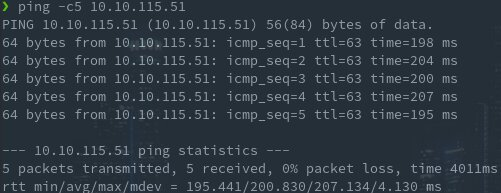
\includegraphics[width=0.8\textwidth]{images/ping.jpg}
	\end{figure}

	\vspace{0.2cm}

	Por el numero del ttl podemos intuir ademas que nos encontramos 
	ante una maquina con Sistema operativo Linux.
	\clearpage
	
	\subsection{Reconocimento de puertos}
	
	Una vez localizado, se realizo un escaneo a traves de la herramienta \textbf{nmap}
	para la deteccion de puertos abiertos.

	% foto del nmap con servicios y scripts basicos
	\begin{figure}[h]
	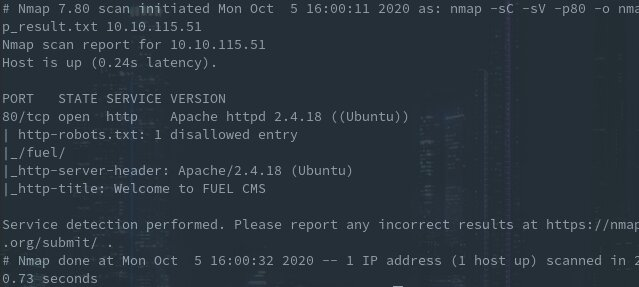
\includegraphics[width=0.8\textwidth]{images/nmap_comun.jpg}
	\end{figure}

	\subsection{Reconocimento Web}
	Una vez dentro nos damos cuenta que la pagina esta utilizando Fuel 
	CMS :
	
	\begin{figure}[h]
   
\includegraphics[width=0.8\textwidth]{images/fuelcms.jpg}
   \end{figure}	
	
	\subsection{Errores encontrados}
	Dentro de su pagina inicial dejaron informacion de la configuracion
	del propio CMS y hasta dejaron credenciales visibles para cualquier
	visitante 
	\\
	Credenciales :
	\begin{figure}[h]
   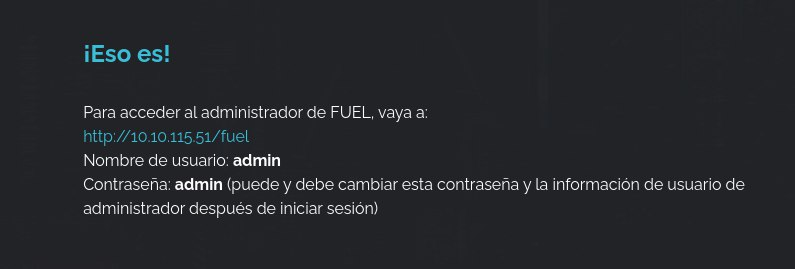
\includegraphics[width=0.8\textwidth]{images/credenciales.jpg}
   \end{figure}


	\vspace{0.2cm}
	\newpage
	Configuracion del CMS :

	\begin{figure}[h]
   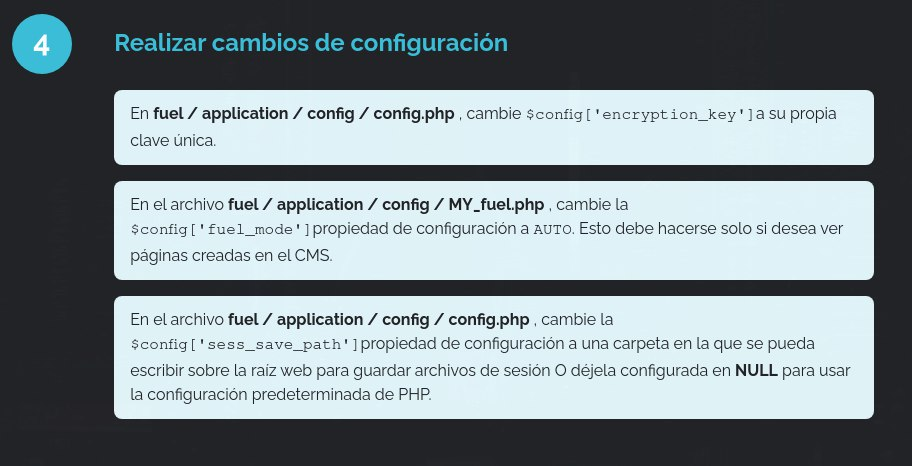
\includegraphics[width=0.8\textwidth]{images/confcms.jpg}
   \end{figure}

	\section{Explotacion}
	Para la parte de explotacion buscamos exploits para fuel cms y
	obtuvimos este resultado :

	\begin{figure}[h]
   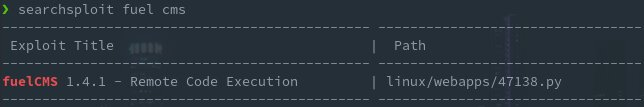
\includegraphics[width=0.8\textwidth]{images/searchsploit.jpg}
   \end{figure}

	\subsection{Exploit}
	El exploit que usamos se basa en una vulnerabilidad de tipo Remote
	Code Execution que apartir de un parametro en la pagina a la que 
	le vamos hacer request nos permite ejecutar comandos, por lo que 
	para usar este exploit tenemos que editar unas cosas minimas para que quede de esta manera.

	\begin{figure}[h]
	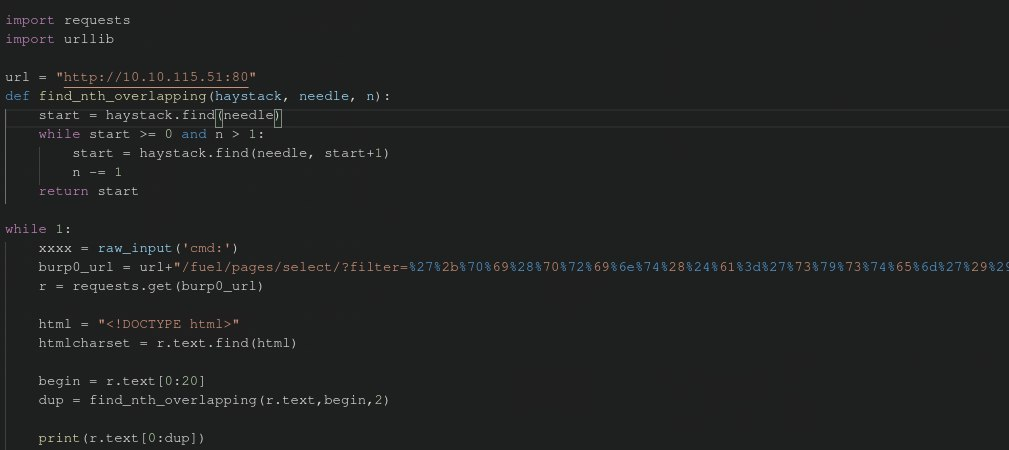
\includegraphics[width=0.8\textwidth]{images/exploit.jpg}
	\end{figure}

	\newpage
	
	\section{Post-Explotacion}
	Una vez dentro de la maquina nos encontramos como usuarios ww-data.
	Por lo que tenemos que escalar privilegios a root pero antes de eso
	podemos capturar la flag.
	 
	\begin{figure}[h]
   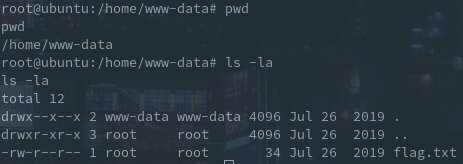
\includegraphics[width=0.8\textwidth]{images/user.jpg}
   \end{figure}

	\subsection{Escala de Privilegios}

	Ahora en la pagina inicial nos dimos cuenta que nos indicaba la
	direccion de los archivos de configuracion del CMS , que tal si
	investigamos por ahi para averiguar que mas podemos encontrar.
	\\
	Y listo encontramos el archivo database.php que contiene estos datos :

	\begin{figure}[h]
   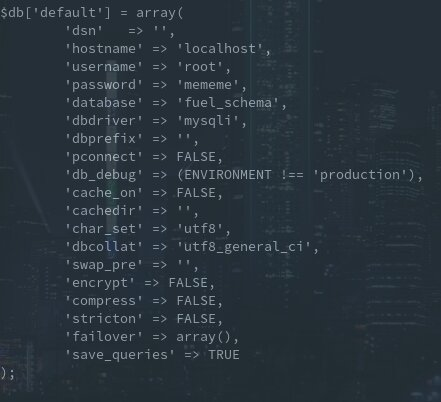
\includegraphics[width=0.8\textwidth]{images/post_ex.jpg}
   \end{figure}
	
	\vspace{0.2cm}
	\newpage
	Una vez hayamos colocado el password y seamos root podemos obtener
	la flag 

	\begin{figure}[h]
   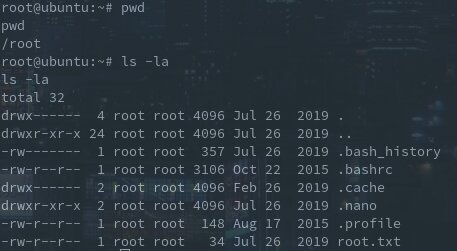
\includegraphics[width=0.8\textwidth]{images/root.jpg}
   \end{figure}
	
	
\end{document}



